%
\section{Design \& Architecture}\label{sec:design_architecture}
%
This chapter will explain the scanner architecture, things that we have considered while designing the component and some of the valuable techniques I have analyzed to make an efficient scanner to extract \acs{OSS} component.

\subsection{Scanner Architecture}
 The first task of developing this scanner is creating an automated \acs{OSS} component extractor because manual extraction of \acs{OSS} component is a tedious and redundant task; finding an automated system will reduce the time consumption and make it more cost-effective. The manual \acs{OSS} extraction is suitable for small projects with less \acs{OSS} components consumption which is a very rare case. The \acs{OSS} scanner is built as a web application in this project by considering some useful advantages like accessibility across the devices, less maintenance and increased flexibility and scalability. Like traditional web applications, the \acs{OSS} scanner has front-end and back-end applications. We have decided to break down the \acs{OSS} scanner into three major parts, which are \acs{OSS} component Analyzer, Evaluator and Reporter. 
 \begin{figure}[h!]
 	\includegraphics[width=15cm]{includes/architetcure.png}
 	\centering
 	\caption{\acs{OSS} scanner architecture}
 	\label{fig:architecture}
 \end{figure}
\newpage
The figure ~\ref{fig:architecture} shows where the three major parts have been placed in the web -application. The \acs{OSS} component analyzer will be developed in the front-end because, as per the research question, the \acs{OSS} components should be scanned in the front-end(web browser). Once the \acs{OSS} components are extracted from the project, the meta-information(name and version) will be sent to the \acs{OSS} component evaluator for finding the vulnerabilities. The \acs{OSS} component evaluator and reporter are developed in the back-end. To make a clear understating, the figure ~\ref{fig:sequence} will show clear interaction between the components.
\begin{figure}[h!]
	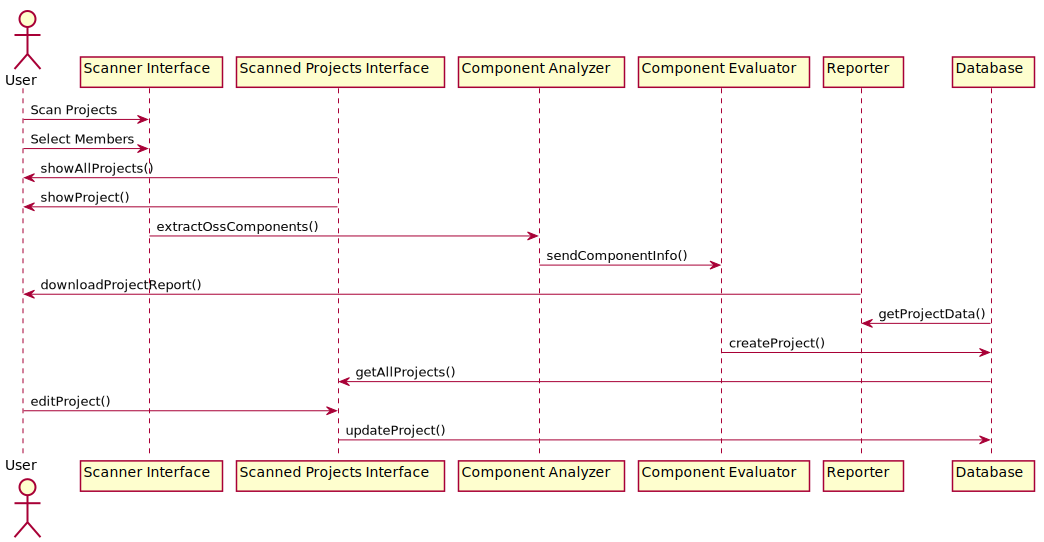
\includegraphics[width=15cm]{includes/sequence_diagram.png}
	\centering
	\caption{\acs{OSS} scanner sequence diagram}
	\label{fig:sequence}
\end{figure} 
\subsection{Scanner Components}

As shown in figure ~\ref{fig:architecture} there are three main components involved in the design and architecture of the \acs{OSS} scanner. Following are the components which are interrelated to each other and gives a big picture of their functionality. \acs{OSS} Component Analyzer, \acs{OSS} Component Evaluator and \acs{OSS} Reporter.

\textbf{\acs{OSS} Component Analyzer:} This component is mainly responsible for extracting the \acs{OSS} components used in the projects. This particular task should be performed on the client-side, where the scanning should take place in the browser. The user's inputs required in this interface are Project name, description, members, and project directory. After receiving the inputs, there are two stages of the automation process. First, the scanner will detect what type of application framework is given as input so that the scanner can parse the targeted file for the further process. Once the target file is parsed, the second process will extract the \acs{OSS} component name and the version used in the project. It creates \acs{JSON} data with basic project information along with the list of \acs{OSS} components and its version. Overall the primary goal of this component is to extract all the \acs{OSS} components, and It will send the data evaluation process.
	
\textbf{\acs{OSS} Component Evaluator:} This component evaluates the \acs{OSS} components which are extracted by the analyzer. The evaluation process component will be developed as a back-end application to perform the process on the server-side. This evaluation is performed with the help of \acs{NVD} database \acs{API} service. The extracted \acs{OSS} components will be searched in the \acs{NVD} database by using its name and version to find the known vulnerabilities registered under the respective component version. This component will be running asynchronously in the server because a project can have n-number of \acs{OSS} components. Once the \acs{OSS} components are evaluated, the information which is collected from the \acs{NVD} database is used for analyzing the risk level of each \acs{OSS} component. Finally, all the information is converted as a \acs{JSON} file and stored as a container in Azure data storage.
	
\textbf{\acs{OSS} Reporter:} This component is a part of the scanner’s user interface where the user can download the \acs{OSS} report of the project. This report shows all the basic information of the project and its \acs{OSS} component along with the vulnerability and the risk level of each component. This component simply generates a pdf report with all the above information retrieved from the database.
	
\subsection{Design Challenge}
Almost every software product development project has a unique set of problems. These issues can be a roadblock to development throughout system design and, more importantly, during implementation. There were several difficulties faced throughout the implementation of this thesis. The major problems that need to be addressed and a solution formed are listed below.

\textbf{Application framework:} Because I had never worked with Angular framework before, the first hurdle I had while starting implementation was familiarizing myself with it. I got acquainted to the Angular environment with the aid of several online tutorials and hands-on programming. The are few reasons why we chose to develop frontend application with  Angular framework because it has faster development process like having neat documentation for understanding Angular with a large developer community and it also helps us with efficient problem-solving patterns where the angular services helps to integrate the business logic with app user-interface.
	
\textbf{File structure:} The next challenge for us was trying to create a generic function that can extract the \acs{OSS} component name version from respected config files of the software project. This challenge was time-consuming because each software project can be built using a different application framework, and also each application framework has its dependency manager. For instance, the Ruby on Rails application framework uses RubyGems as a dependency manager. The Ruby on Rails application framework generates a file called Gemfile, where all the required dependencies of the project will be mentioned there along with the version of the dependency. The file type of the Gemfile is .gemfile.  Likewise, each application framework has a different file type as refereed in the table ~\ref{tab:configFiles}. To overcome this challenge, when the project data is submitted at the beginning, the project data should pass a condition to identify which application framework it is. Once identifying the application, the OSS component extraction will be performed based on the file type of config file. So for each application framework, there should be different extraction functions. 
		
\textbf{Finding the right regex:} Another challenge was finding the correct regex for each config file. The more challenging part was extracting the \acs{OSS} component names and versions from config files like Gemfile and requirements.txt. It was not that difficult to overcome this challenge because the same solution, like the file structure, is required for this challenge. When the user submits a Django or Ruby on Rails project, firstly, as we said, the condition will identify the application framework and based on the file type, the extraction will be performed. The regex is implemented in the extraction function, for instance, when we see the figure ~\ref{fig:ruby} which lists all the OSS components used in a Ruby on Rails project. Each file line will be sent for a cleaning process and delivers the component name and version, which is extracted from each line. To extract the name and version from each line, a proper regex is required. Like Django and Ruby on Rails, the other application framework was not that difficult because most file types were XML and JSON files. The component name version can be easily extracted with the help of JSON and XML DOM parsing functions.  
	
\textbf{Result Verification: }Another issue was determining whether what we built corresponded to what was happening within the software. To do so, we ran our code on a set of test projects whose results were already known and checked if our application produced the same results. If the results come as not expected, then we must do code modification in the component analyzer. So, therefore, for each application framework project, few modifications will be performed until we receive the expected output.

%
